% We will describe the spectral embedding,  

% ------------------------

% nonlinear dimension reduction:
% 1. construct a neighborhood graph G and compute similarity matrix S ($\sigma$ controls neighborhood size)
% 2. derive Laplacian matrix L (symmetric) from S
% 3. perform embedding algorithm; ouput: s-dimensional representation $y_i$ corresponding to each data point $x_i$
% 4. estimate the distortion incurred w.r.t the original data. 

% a generated dataset of our own, 

\textbf{Our generated dataset} \cite{swiss-roll}

The Swiss roll dataset was created in 2004 to use for testing dimensionality reduction techniques. It is now a commonly used toy dataset in scikit-learn. Consisting of a set of three-dimensional points arranged in a "roll" shape, the dataset resembles the Swiss roll cake which is the origin of the dataset's name. This can be seen in Fig. \ref{fig:swiss-roll}. The points on the dataset are colored a lot of the time, making it easier to visualize the plot of the reduced data. What made the Swiss roll dataset popular is its easy generation and visualisation along with its nonlinear structure - in contrast to the linear dimensionality reduction methods, e.g. PCA. \\

\begin{figure}[H]
    \centering
    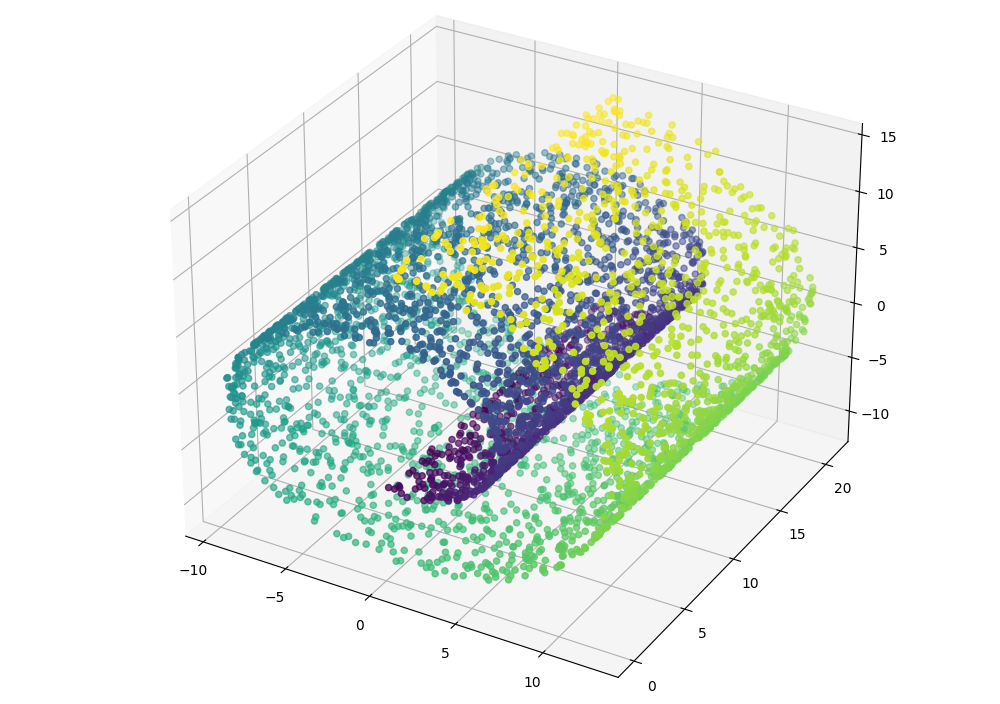
\includegraphics[width=0.6\textwidth]{images/swissRoll5000.png}
    \caption{Swiss roll with 5000 datapoints}
    \label{fig:swiss-roll}
\end{figure}

% The Swiss roll is a toy dataset in scikit learn that is commonly used for testing and demonstrating nonlinear dimensionality reduction algorithms. It consists of a set of points in three dimensions, arranged in a “roll” shape, such that the points on the roll are mapped to a two-dimensional plane in a nonlinear fashion. The points on the Swiss roll are often colored so that the resulting plot of the reduced data can be visualized more easily.

% The Swiss roll dataset is often used because it is easy to generate and visualize, and because it exhibits a nonlinear structure that is not captured by linear dimensionality reduction methods such as PCA. It is also a useful benchmark for comparing the performance of different nonlinear dimensionality reduction algorithms.

% ----

% The Swiss Rolls dataset is a simple 1600 x 3 dimension dataset. It consists of 1600 observations of 3 variables which represent 3-dimensional coordinates. The Swiss roll dataset appears to have been created in 2004 by Dinoj Surendran while he was studying at the University of Chicago.

% His intended purpose of creating the data set was to use it for testing dimensionality reduction techniques. It gets its name due to the.. looks uncannily similar to the dessert snack "Swiss Rolls". 


% and both real-world-based datasets Word2Vec 

\textbf{Word2Vec} \cite{mikolov2013efficient}  

As there are many different types of similarities between words, it is sensible to use high-dimensional word vectors. Mikolov et al. discovered that simple algebraic operations can be performed using these vector representations. For example, there could be a given word pair (a, b) that holds a distinct difference. Using algebra, a word X can be found holding the same difference to a given word (c): \\

X = a - b + c \\

For example (see Fig. \ref{fig:word2vec}): \\
vector("king") = vector("man") - vector("woman") + vector("queen") \\
vector("smallest") = vector("biggest") - vector("big") + vector("small") \\

\begin{figure}[H]
    \centering
    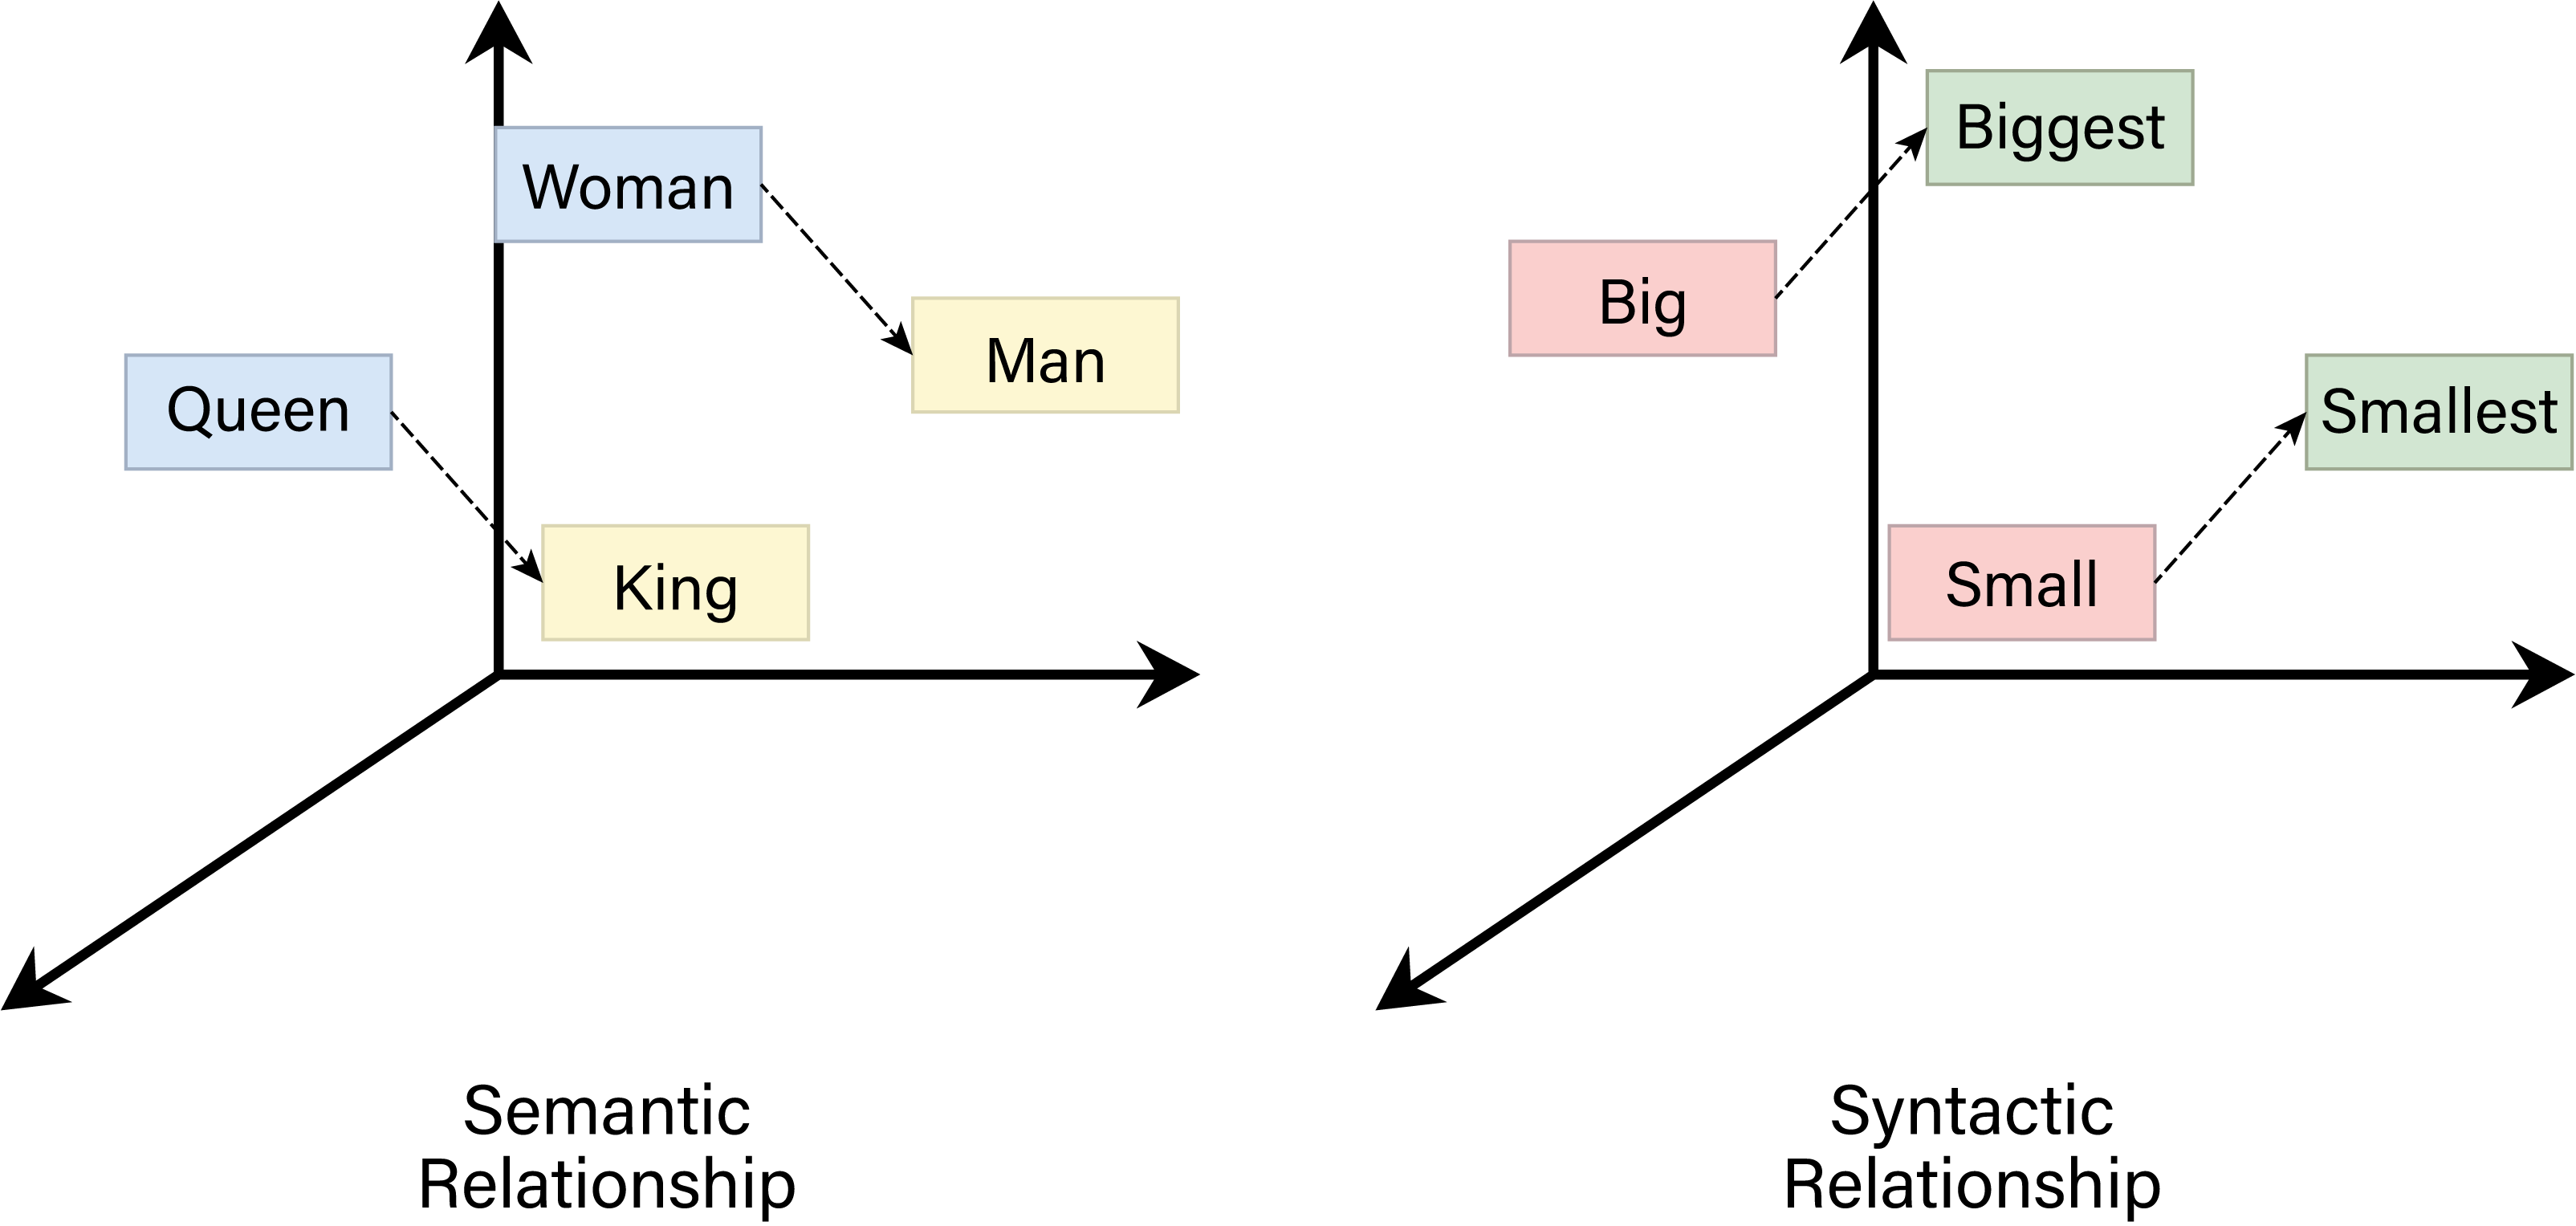
\includegraphics[width=0.6\linewidth]{images/word2vec.png}
    \caption{Semantic and Syntactic Relationships in Word2Vec}
    \label{fig:word2vec}
\end{figure}

When high-dimensional word vectors are trained on a large amount of data, very subtle semantic relationships between words can be discovered. Next to semantic similarities, the team of Google also looked at the words in the context of syntactic similarities. Several tests were run on different simple model architectures and compared on accuracy. As a result of one test, the team realized that using multiple examples instead of just one to form the relationship vector improved the accuracy of the best models by about 10\% absolutely on the semantic-syntactic test. The models were all implemented in a distributed framework titled DistBelief; they were trained on the Google News 6B data set, with mini-batch asynchronous gradient descent and Adagrad. After the first publication of the paper, Mikolov et al. published code for computing the word vectors with an improved training speed as well as more than 1.4 million vectors of dimensionality 300 representing named entities, trained on more than 100 billion words. The Word2Vec dataset now is one of the most popular implementations of word embedding and has been commonly used throughout its existing years. \\

% ------------

% vector("nephew") = vector("brother") - vector("sister") + vector("niece") \\
% vector("smallest") = vector("biggest") - vector("big") + vector("small") \\

% there can be many different types of similarities between words

% Somewhat surprisingly, these questions can be answered by performing simple algebraic operations with the vector representation of words. To find a word that is similar to small in the same sense as biggest is similar to big, we can simply compute vector X = vector("biggest")-vector("big")+vector("small"). Then, we search in the vector space for the word closest to X measured by cosine distance and use it as the answer to the question

% Finally, we found that when we train high-dimensional word vectors on a large amount of data, the resulting vectors can be used to answer very subtle semantic relationships between words

% semantic questions, syntactic questions

% By using ten examples instead of one to form the relationship vector (we average the individual vectors together), we have observed an improvement in accuracy of our best models by about 10\% absolutely on the semantic-syntactic test.

% As mentioned earlier, we have implemented various models in a distributed framework called DistBelief. Below we report the results of several models trained on the Google News 6B data set, with mini-batch asynchronous gradient descent and the adaptive learning rate procedure called Adagrad

% train high-quality word vectors using very simple model architectures

% we published single-machine multi-threaded C++ code for computing the word vectors, using both the continuous bag-of-words and skip-gram architectures. The training speed is significantly higher than reported earlier in this paper, i.e. it is in the order of billions of words per hour for typical hyperparameter choices. We also published more than 1.4 million vectors that represent named entities, trained on more than 100 billion words.


% and Galaxies used in the paper.

\textbf{Galaxy spectra} \cite{galaxies} \cite{Spectra}

Next to Word2Vec, Megaman also used galaxy spectra from the Sloan Digital Sky Survey (SDSS). While it is not specified in the paper, according to the year of publication, the data is likely to be from the SDSS-III release. \\

SDSS made it their mission to observe stars, galaxies, and quasars and provide the world with near-continuos data. So far, there have been five phases. The first one, SDSS-I, dates back to 2000. Among other things, optical spectra of more than 700,000 objects were collected. SDSS-III was published in 2011 and put its focus on spectroscopy. Their survey required an upgrade to optical spectrographs. Additionally, infrared spectrographs were introduced. \\

The spectrum of a galaxy represents the emitted or absorbed light across a range of wavelengths from the various objects within that galaxy. It provides information about the composition, temperature, density, and motion of the contributing astronomical entities within the galaxy. The spectrum is a valuable tool for astronomers to study the characteristics and properties of galaxies. \\

In the Megaman paper, an article is referred to view the preprocessing of this galaxy spectra data. However, it is stated to be "in preparation" and we could not find a publication. Therefore, we decided to focus on the Word2Vec dataset used in the paper. 